\documentclass[12pt, letterpaper]{article}

\usepackage{amsmath}
\usepackage[a4paper, portrait, margin=1in]{geometry}
\usepackage{hyperref}
\usepackage{minted}
\usepackage{mdframed}
\usepackage{tikz}
\usepackage{listings}
\usepackage{multirow}
\usepackage{bookmark}
\usepackage{xcolor}
\usepackage{colortbl}
\usepackage{framed}

\definecolor{shadecolor}{RGB}{240,240,240}
\newcommand{\mybox}[1]{\par\noindent\colorbox{shadecolor}
{\parbox{\dimexpr\textwidth-2\fboxsep\relax}{#1}}}

\renewcommand{\thesection}{Question \arabic{section}}
\renewcommand{\thesubsection}{\arabic{section}\alph{subsection})}
\renewcommand{\thesubsubsection}{\roman{subsubsection})}
\renewcommand{\thefigure}{\arabic{figure}}

\lstset{
basicstyle=\small\ttfamily,
columns=flexible,
breaklines=true
}

\hypersetup{
    colorlinks=true,
    linkcolor=blue,
    filecolor=magenta,      
    urlcolor=blue,
}

\setlength{\parindent}{0em}
\setlength{\parskip}{1em}


\title{CSS601 Introduction to Artificial Intelligence - Assignment 2}
\author{Ian Chong Wei Ming\\
\href{mailto:ian.chong.2020@mitb.smu.edu.sg}{ian.chong.2020@mitb.smu.edu.sg}\\
+65-9680-8118}
\date{\today}

\begin{document}

\maketitle

\mybox{\textbf{Note:} Given information will be shaded \underline{grey} or in \textit{tables}.}

\section{Heuristic Search}
\begin{center}
    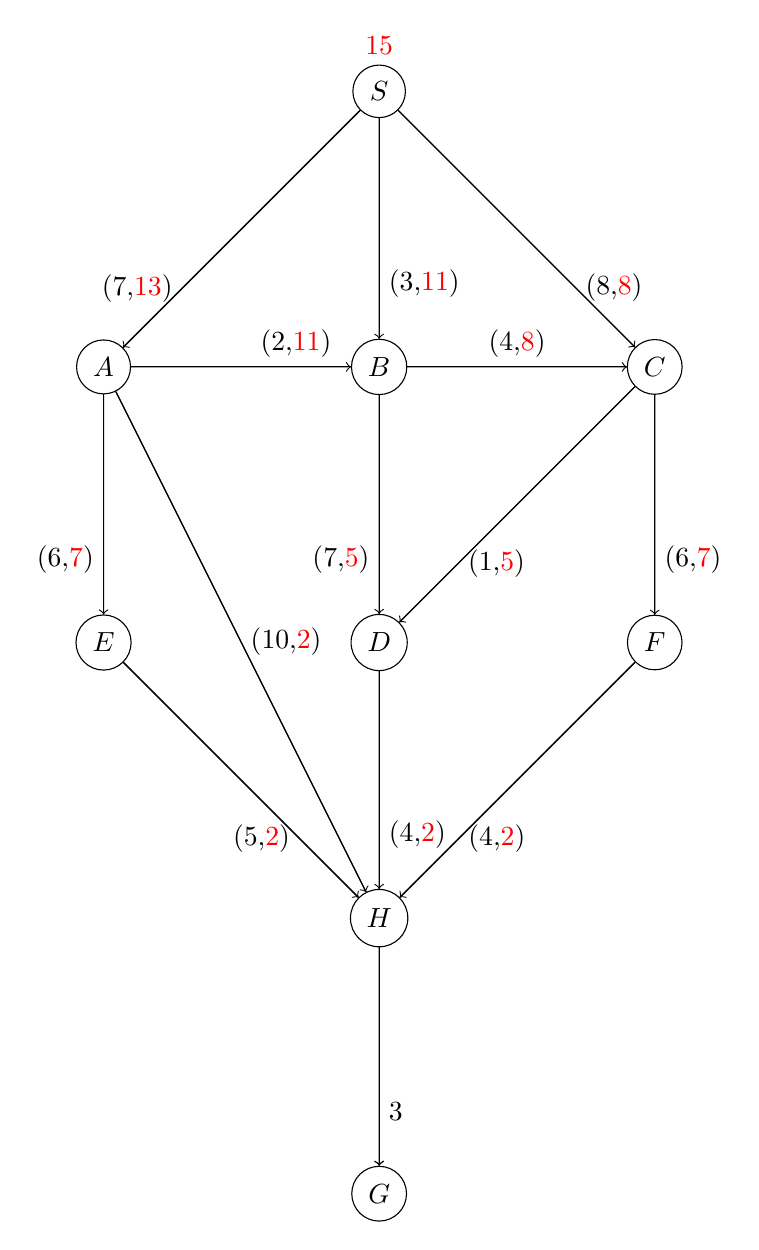
\begin{tikzpicture}[node distance=3.5cm]
        
        \node[circle,draw,label={\textcolor{red}{15}}] (S) {$S$};
        \node[circle,draw, below of=S] (B) {$B$};
        \node[circle,draw, left of=B] (A) {$A$};
        \node[circle,draw, right of=B] (C) {$C$};
        \node[circle,draw, below of=B] (D) {$D$};
        \node[circle,draw, below of=A] (E) {$E$};
        \node[circle,draw, below of=C] (F) {$F$};
        \node[circle,draw, below of=D] (H) {$H$};
        \node[circle,draw, below of=H] (G) {$G$};
    
        \path [->,draw] 
        (S) -- (B)
        (S) -- (A)
        (S) -- (C)
        (A) -- (B)
        (A) -- (E)
        (A) -- (H)
        (B) -- (C)
        (B) -- (D)
        (C) -- (D)
        (C) -- (F)
        (E) -- (H)
        (D) -- (H)
        (F) -- (H)
        (H) -- (G);
    
        \path[->,draw]
        (S) edge node[right, near end] {(3,\textcolor{red}{11})} (B)
        (S) edge node[left, near end] {(7,\textcolor{red}{13})} (A)
        (S) edge node[right, near end] {(8,\textcolor{red}{8})} (C)
        (A) edge node[above, near end] {(2,\textcolor{red}{11})} (B)
        (A) edge node[left, near end] {(6,\textcolor{red}{7})} (E)
        (A) edge node[right] {(10,\textcolor{red}{2})} (H)
        (B) edge node[above] {(4,\textcolor{red}{8})} (C)
        (B) edge node[left, near end] {(7,\textcolor{red}{5})} (D)
        (C) edge node[right, near end] {(1,\textcolor{red}{5})} (D)
        (C) edge node[right, near end] {(6,\textcolor{red}{7})} (F)
        (E) edge node[left, near end] {(5,\textcolor{red}{2})} (H)
        (D) edge node[right, near end] {(4,\textcolor{red}{2})} (H)
        (F) edge node[right, near end] {(4,\textcolor{red}{2})} (H)
        (H) edge node[right, near end] {3} (G);
    \end{tikzpicture}
\end{center}

\mybox{For the above graph (heuristic values are provided in red color and actual costs are in black
color), please provide answers to the following answers. Also note that S is start state and G
is goal state.}

\subsubsection{Is the heuristic admissible?}

\textbf{Response:} A heuristic is defined as \textit{admissible} if it never \textit{overestimates} the \textbf{cost} of reaching the \textbf{goal}. 
In otherwords, the cost that estimated by the heuristic to reach the goal \textbf{cannot} be \textit{higher} than the \textit{lowest} possible cost from the \textit{current point} in the path.
More formally, $h(n)\leq c(n,g) \forall n$

The minimum cost and the heuristic $h(n)$ to reach the goal from each node is given in the following table.
Workings will follow the table.

\begin{center}
    \begin{tabular}{|c|c|c|c|} 
    \hline
    Node $n$ & $c(n,g)$ & $h(n)$ & $h(n)\leq c(n,g)?$ \\ 
    \hline
    S & 15 & 15 & TRUE\\
    \hline
    A & 13 & 13 & TRUE\\
    \hline
    B & 12 & 11 & TRUE\\
    \hline
    C & 8 & 8 & TRUE\\
    \hline
    E & 8 & 7 & TRUE\\
    \hline
    D & 7 & 5 & TRUE\\
    \hline
    F & 7 & 7 & TRUE\\
    \hline
    H & 3 & 2 & TRUE\\
    \hline
    \end{tabular}
\end{center}

\textbf{Node S}

The path to follow would be $S\rightarrow B\rightarrow C\rightarrow D\rightarrow H\rightarrow G$

$c(n,g)=3+4+1+4+3=\underline{\textbf{15}}$

$h(n)=\textcolor{red}{15}$

\textbf{Node A}

The path to follow would be $A\rightarrow H\rightarrow G$

$c(n,g)=\underline{\textbf{13}}$

$h(n)=\textcolor{red}{13}$

\textbf{Node B}

The path to follow would be $B\rightarrow C\rightarrow D\rightarrow H\rightarrow G$

$c(n,g)=4+4+1+3=\textbf{\underline{12}}$

$h(n)=\textcolor{red}{11}$

\textbf{Node C}

The path to follow would be $C\rightarrow D\rightarrow H\rightarrow G$

$c(n,g)=1+4+3=\underline{\textbf{8}}$

$h(n)=\textcolor{red}{8}$

\textbf{Node D}

The path to follow would be $D\rightarrow H\rightarrow G$

$c(n,g)=4+3=\underline{\textbf{7}}$ 

$h(n)=\textcolor{red}{5}$

\textbf{Node E}

The path to follow would be $E\rightarrow H\rightarrow G$

$c(n,g)=5+3=\underline{\textbf{8}}$ 

$h(n)=\textcolor{red}{7}$

\textbf{Node F}

The path to follow would be $F\rightarrow H\rightarrow G$

$c(n,g)=4+3=\underline{\textbf{7}}$ 

$h(n)=\textcolor{red}{7}$

\textbf{Node H}

The path to follow would be $H\rightarrow G$

$c(n,g)=\underline{\textbf{3}}$ 

$h(n)=\textcolor{red}{2}$

Since $h(n)\leq c(n,g) \forall n$, the heuristic is \textit{admissible}.

\subsubsection{Is the heuristic consistent? Provide justification}
\textbf{Response:} No, the heuristic is not \textit{consistent}.

A heuristic is \textit{consistent} only if its estimate is \underline{always} less than or equal to the estimated distance from any neighbouring vertex to the goal, plus the cost of reaching that neighbour. More formally:

\[h(n) \leq c(n,p) + h(p) \forall n\]

Non-consistent nodes in the following table are coloured \colorbox{red}{RED}


\begin{center}
    \begin{tabular}{|c|c|c|c|} 
    \hline
    Node $n$ & $h(n)$ & $p$ & $c(n,p)+h(p)$ \tabularnewline
    \hline
    S & 15 & A & 20\tabularnewline
    \hline
    \rowcolor{red}S & 15 & B & 14\tabularnewline
    \hline
    S & 15 & C & 16\tabularnewline
    \hline
    A & 13 & B & 13\tabularnewline
    \hline
    A & 13 & E & 13\tabularnewline
    \hline
    \rowcolor{red}A & 13 & H & 12\tabularnewline
    \hline
    B & 11 & C & 12\tabularnewline
    \hline
    B & 11 & D & 12\tabularnewline
    \hline
    \rowcolor{red}C & 8 & D & 6\tabularnewline
    \hline
    C & 8 & F & 13\tabularnewline
    \hline
    D & 5 & H & 6\tabularnewline
    \hline
    E & 7 & H & 7\tabularnewline
    \hline
    \rowcolor{red}F & 7 & H & 6\tabularnewline
    \hline
    H & 2 & G & 3\tabularnewline
    \hline

    \end{tabular}
\end{center}

\subsubsection{DFS, BFS, Best First Search and A* Search}
\mybox{Provide the search steps (as discussed in class) with DFS, BFS (with and without priority
queue), Best First Search and A* search. Specify for each algorithm if the open list is
queue, stack, or priority queue. Feel free to add rows/columns, or other details in the
table below. Open list contains nodes that are to be explored, and “Nodes to add” are
the successors of the node that is recently popped.}

\textbf{Response:} The following tables detail the steps each algorithm takes.

\begin{center}
    \begin{tabular}{|c|c|c|c|}
    \hline
    \multicolumn{4}{|c|}{Depth First Search (\textbf{DFS})\textcolor{red}{*}}\\
    \hline
    Step No. & Open List & POP & Nodes to add \\ 
    \hline
    1 & $S$ & $S$ & $A^S, B^S, C^S$ \\
    \hline
    2 & $A^S, B^S, C^S$ & $A^S$ & $E^A,H^A$ \\
    \hline
    3 & $E^A, H^A, B^S, C^S$ & $E^A$ & nil \\
    \hline
    4 & $H^A, B^S, C^S$ & $H^A$ & $G^H$ \\
    \hline
    5 & $G^H,B^S,C^S$ & $G^H$ & nil \\
    \hline
    \end{tabular}
\end{center}

\textcolor{red}{*Open List is a \textit{stack}}

The path to follow is $S\rightarrow A\rightarrow H\rightarrow G$

Cost = 7 + 10 + 3 = \underline{\textbf{20}}

\begin{center}
    \begin{tabular}{|c|c|c|c|}
    \hline
    \multicolumn{4}{|c|}{Breadth First Search (\textbf{BFS})}\\
    \hline
    Step No. & Open List\textcolor{red}{*} & POP & Nodes to add \\ 
    \hline
    1 & $S$ & $S$ & $A^S, B^S, C^S$ \\
    \hline
    2 & $A^S, B^S, C^S$ & $A^S$ & $E^A,H^A$ \\
    \hline
    3 & $B^S, C^S, E^A, H^A$ & $B^S$ & $D^B$ \\
    \hline
    4 & $C^S, E^A, H^A, D^B$ & $C^S$ & $F^C$ \\
    \hline
    5 & $E^A,H^A,D^B,F^C$ & $E^A$ & nil \\
    \hline
    6 & $H^A,D^B,F^C$ & $H^A$  & $G^H$ \\
    \hline
    7 & $D^B,F^C,G^H$ & $D^B$  & nil \\
    \hline
    8 & $F^C,G^H$ & $F^C$  & nil \\
    \hline
    9 & $G^H$ & $G^H$  & nil \\
    \hline
    \end{tabular}
\end{center}

\textcolor{red}{*Open List is a \textit{queue}}

The path to follow is $S\rightarrow A\rightarrow H\rightarrow G$

Cost = 7 + 10 + 3 = \underline{\textbf{20}}

\begin{center}
    \begin{tabular}{|c|c|c|c|}
    \hline
    \multicolumn{4}{|c|}{Breadth First Search (\textbf{BFS} - Optimal)}\\
    \hline
    Step No. & Open List\textcolor{red}{*} & POP & Nodes to add \\ 
    \hline
    1 & $S$ & $S$ & $B^{S,3}, A^{S,7}, C^{S,8}$\\
    \hline
    2 & $B^{S,3}, A^{S,7}, C^{S,8}$ & $B^{S,3}$ & $C^{B,7},D^{B,10}$ \\
    \hline
    3 & $A^{S,7}, C^{B,7}, D^{B,10}$ & $A^{S,7}$ & $E^{A,13}, H^{A,17}$ \\
    \hline
    4 & $C^{B,7}, D^{B,10}, E^{A,13}, H^{A,17}$ & $C^{B,7}$ & $D^{C,8}, F^{C,13}$\\
    \hline
    5 & $D^{C,8}, E^{A,13}, F^{C,13}, H^{A,17}$ & $D^{C,8}$ & $H^{D,12}$\\
    \hline
    6 & $H^{D,12}, E^{A,13}, F^{C,13}$ & $H^{D,12}$ & $G^{H,15}$\\
    \hline
    7 & $E^{A,13}, F^{C,13}, G^{H,15}$ & $E^{A,13}$ & $H^{E,18}$\textcolor{red}{**}\\
    \hline
    8 & $F^{C,13}, G^{H,15}$ & $F^{C,13}$ & $H^{F,18}$\textcolor{red}{**}\\
    \hline
    9 & $G^{H,15}$ & $G^{H,15}$ & nil\\
    \hline
    \end{tabular}
\end{center}

\textcolor{red}{*Open List is a \textit{priority queue}}

\textcolor{red}{**not added to the Open list since it is already \textit{explored}}

The path to follow is $S\rightarrow B\rightarrow C\rightarrow D\rightarrow H\rightarrow G$

Cost = 3 + 4 + 1 + 4 + 3 = \underline{\textbf{15}}

\begin{center}
    \begin{tabular}{|c|c|c|c|}
    \hline
    \multicolumn{4}{|c|}{Best First Search}\\
    \hline
    Step No. & Open List\textcolor{red}{*} & POP & Nodes to add \\ 
    \hline
    1 & $S$ & $S$ & $A^{S,13}, B^{S,11}, C^{S,8}$ \\
    \hline
    2 & $C^{S,8}, B^{S,11}, A^{S,13}$ & $C^{S,8}$ & $D^{C,5}, F^{C,7}$ \\
    \hline
    3 & $D^{C,5}, F^{C,7}, B^{S,11}, A^{S,13}$ & $D^{C,5}$ & $H^{D,2}$ \\
    \hline
    4 & $H^{D,2}, F^{C,7}, B^{S,11}, A^{S,13}$ & $H^{D,2}$ & $G^{H,0}$\\
    \hline
    5 & $G^{H,3}, F^{C,7}, B^{S,11}, A^{S,13}$ & $G^{H,0}$ & nil\\
    \hline
    \end{tabular}
\end{center}

\textcolor{red}{*Open List is a \textit{queue}}

The path to follow is $S\rightarrow C\rightarrow D\rightarrow H\rightarrow G$

Cost = 8 + 1 + 4 + 3 = \underline{\textbf{16}}

\begin{center}
    \begin{tabular}{|c|c|c|c|}
    \hline
    \multicolumn{4}{|c|}{A* Search}\\
    \hline
    Step No. & Open List\textcolor{red}{*} & POP & Nodes to add \\ 
    \hline
    1 & $S$ & $S^{15}$ & $B^{S,14}, C^{S,16}, A^{S,20}$ \\
    \hline
    2 & $B^{S,14}, C^{S,16}, A^{S,20}$ & $B^{S,14}$ & $C^{B,15}, D^{B,15}$ \\
    \hline
    3 & $C^{B,15}, D^{B,15}, A^{S,20}$ & $C^{B,15}$ & $D^{C,13},F^{C,20}$ \\
    \hline
    4 & $D^{C,13}, A^{S,20}, F^{C,20}$ & $D^{C,13}$ & $H^{D,14}$\\
    \hline
    5 & $H^{D,14}, A^{S,20}, F^{C,20}$ & $H^{D,14}$ & $G^{H,15}$\\
    \hline
    6 & $G^{H,15}, A^{S,20}, F^{C,20}$ & $G^{H,15}$ & nil\\
    \hline
    \end{tabular}
\end{center}

\textcolor{red}{*Open List is a \textit{priority queue}}

The path to follow is $S\rightarrow B\rightarrow C\rightarrow D\rightarrow H\rightarrow G$

Cost = 3 + 4 + 1 + 4 + 3 = \underline{\textbf{15}}

\section{Build an automated car in a simulator}

\mybox{The goal of this assignment is to guide your car to move in a multi-lane straight road (represented using a rectangular grid) simulator (details explained later). 

In addition to your car, there are other cars also moving along the road. You need to design an algorithm which can take your car from its start position to the end of the road as soon as possible while avoiding other cars. 

Other cars are moving randomly. At any step, your car can view up to 4 cells in front, left and right, i.e., it will not be able to look at the other cars which are beyond its visibility range of 4 cells. (This visibility range of 4 is configurable and your algorithm should work irrespective of visibility range).

We describe the state, operators and goal state for this problem below.

\textbf{State}: State of the car is its location, i.e., the grid cell it is currently present in. 

\textbf{Operators/Actions}: Following are the available operators or actions for the car:

\begin{itemize}
    \item \textbf{Forward} – Moves the car one step ahead in the same lane.
    \item \textbf{Forward-2$\times$} – Moves the car two steps ahead in the same lane.
    \item \textbf{Forward-3$\times$} – Moves the car three steps ahead in the same lane.
    \item \textbf{Left} – Moves the car in the left lane and one step forward.
    \item \textbf{Right} – Moves the car in the right lane and one step forward.
    \item \textbf{None} – Stays at the same place.
\end{itemize}

If the action is unsuccessful then the car will stay at the same place. Action will be unsuccessful if there is a wall or another car present in the intended direction of move. For example, a forward will be unsuccessful if there is another car present in front of your car.
As the left action moves a car to the left and one step forward, a left action taken in grid cell (5,3) will be unsuccessful if there is a car in either of (4,3) or (4,4).

\textbf{Goal State:} There is one goal state, where your car needs to reach.}

\subsection{Write the function}
\mybox{Write the function that will generate the \textbf{operator/action} to be taken at the current time step (based on search algorithms discussed in class), so that time taken to reach goal is as \textit{minimal} as possible. 
[You may refer to “\texttt{pseudo code.pdf}” for implementation details and pseudo code for $A* Search$.]
The code for the Simulator is provided in the zip file \texttt{"SelfDrivingCar.zip"}. The details about the
installation/running of simulator and code details are provided in the file \texttt{"SelfDrivingCar.pdf"}
(present in the \texttt{.zip} file).}

\textbf{Response:} Please see attached \texttt{python} script.

\subsection{Submit code in \texttt{.pdf}}

\textbf{Response:}

\subsubsection{Algorithm 1 - \texttt{drive}}

This is the code for the main drive code. It depends on the subsequent helper functions.

\begin{mdframed}[backgroundcolor=shadecolor]
\begin{minted}[fontsize=\footnotesize,breaklines]{python}
def drive(self, goalstates, inputs):    
    
    path_list = []
    destination_reached = []
    action_order = []
    path_lengths = []
    start = self.state

    for goal in goalstates:
        goalReached, path = self.AStar(start["location"], goal, inputs)
        destination_reached.append(goalReached)
        path_list.append(path)
        path_lengths.append(len(path))
    
    if True in destination_reached:        
        best_path = [path_list[i] for i in range(len(path_list)) if (destination_reached[i] == True) and (len(path_list[i]) == min(path_lengths))]
        action_order.extend(best_path)
    else:        
        longest_path = [path_list[i] for i in range(len(path_list)) if (len(path_list[i]) == max(path_lengths))]
        action_order.extend(longest_path)

    movements = {
        (0, 3): "forward-3x", 
        (0, 2): "forward-2x", 
        (0, 1): "forward", 
        (-1, 1): "left", 
        (1, 1): "right", 
        (0, 0): None}
    try:
        action_sequence = [movements[(action_order[0][i+1][0] - action_order[0][i][0], action_order[0][i+1][1] - action_order[0][i][1])] for i in range(len(action_order[0])-1)]
    except:
        action_sequence = [None]
    
    return action_sequence
\end{minted}
\end{mdframed}

\subsubsection{Algorithm 2 - \texttt{AStar}}

Implementation of $A* Search$ to car to consider which action to take. Relies on \texttt{applyAction} to function properly.

\begin{mdframed}[backgroundcolor=shadecolor]
\begin{minted}[fontsize=\footnotesize,breaklines]{python}
def AStar(self, start, goal, state):    
    closedSet = []
    openSet = [start]
    cameFrom = {}
    gScore = {start: 0}
    fScore = {start: self.heuristic_cost_estimate(start, goal)}
    current = []
    
    while len(openSet) > 0:
        min_idx = list(fScore.values()).index(min(fScore.values()))
        current = list(fScore.keys())[min_idx]
        if current == goal["location"]:
            return True, self.reconstruct_path(cameFrom, current)
        del fScore[current]
        openSet.remove(current)
        closedSet.append(current)
        
        for action in ["forward-3x", "forward-2x", "forward", "left", "right"]:
            neighbor = self.applyAction(current, action, state, goal["location"])
            if neighbor == current:
                continue
            tentative_gScore = gScore[current] + 1
            if neighbor not in openSet:
                openSet.append(neighbor)
            elif tentative_gScore >= gScore[neighbor]:
                continue
            cameFrom[neighbor] = current
            gScore[neighbor] = tentative_gScore
            fScore[neighbor] = gScore[neighbor] + self.heuristic_cost_estimate(neighbor, goal)
        
    if current == goal["location"]:
        return True, self.reconstruct_path(cameFrom, current)
    else:
        return False, self.reconstruct_path(cameFrom, current)
\end{minted}
\end{mdframed}

\subsubsection{Algorithm 2.5 - \texttt{applyAction}}

Helper function to determine if a move is valid and apply it. For invalid moves, returns the current position \textit{i.e.} no action

\begin{mdframed}[backgroundcolor=shadecolor]
\begin{minted}[fontsize=\footnotesize,breaklines]{python}
def applyAction(self, current, action, state, goal):
    movements = {
        "forward-3x": [(0, 1), (0, 2), (0, 3)], 
        "forward-2x": [(0, 1), (0, 2)], 
        "forward": [(0, 1)], 
        "left": [(-1, 0), (-1, 1)], 
        "right": [(1, 0), (1, 1)], 
        None: [(0, 0)]}
    
    target_row = current[0]
    target_col = current[1]
    valid_move = True
    
    for movement in movements[action]:
        if (target_row + movement[0] >= len(state)) or \
            (target_row + movement[0] < 0) or \
            (target_col + movement[1]) >= len(state[0]):
            return current
                
        if state[target_row + movement[0]][target_col + movement[1]] == 1:
            valid_move = False
            break
        
    if abs(target_row + movements[action][-1][0] - goal[0]) > abs(goal[1] - (target_col + movements[action][-1][1])):
        return current
    
    if valid_move:
        target_row += movements[action][-1][0]
        target_col += movements[action][-1][1]
    return (target_row, target_col)
\end{minted}
\end{mdframed}

\subsubsection{Algorithm 3 - \texttt{heuristic\_cost\_estimate}}

Estimates the heuristic cost from current node.

\begin{mdframed}[backgroundcolor=shadecolor]
\begin{minted}[fontsize=\footnotesize,breaklines]{python}
def heuristic_cost_estimate(self, start, goal):
    result = abs(goal["location"][1] - start[1]) + abs(goal["location"][0] - start[0]) / 2
    return result
\end{minted}
\end{mdframed}

\subsubsection{Algorithm 4 - \texttt{reconstruct\_path}}

Helper function to reconstruct the path from start to current node.

\begin{mdframed}[backgroundcolor=shadecolor]
\begin{minted}[fontsize=\footnotesize,breaklines]{python}
def reconstruct_path(self, cameFrom, current):
    total_path = []
    while current in cameFrom.keys():
        total_path.append(current)
        current = cameFrom[current]
    total_path.append(current)
    total_path = total_path[::-1]
    return total_path
\end{minted}
\end{mdframed}

\section{Taxi Driver Markov Decision Process}
\mybox{Taxi drivers in Singapore can pick up customers from any location that is not on highways. 
However, they require guidance on where to pick up customers when they do not have customers on board and there are no bookings. 
In this question, we address this guidance problem. 
There are four locations: $L1$, $L2$, $L3$ and $L4$ from where taxi drivers can pick up and drop off customers. 
At any decision epoch, the chances of the taxi driver picking up a customer from different locations are provided in \textbf{Table 1} below:}

\begin{center}
    \textbf{Table 1}

    \begin{tabular}{|c|c|} 
    \hline
    Location & Chance of finding customer\\ 
    \hline
    $L1$ & 0.3 \\
    \hline
    $L2$ & 0.8 \\
    \hline
    $L3$ & 0.1 \\
    \hline
    $L4$ & 0.6 \\
    \hline
    \end{tabular}
    
\end{center}

\mybox{Once the taxi driver picks up a customer, the customer determines the destination. Observed
probabilities (from past data) of a customer starting from a source location and going to a
destination location are given below:}

\begin{center}
    \textbf{Table 2}

    \begin{tabular}{|c|c|} 
    \hline
    $Source \rightarrow Destination$ & Probability\\ 
    \hline
    $L1 \rightarrow L2$ & 0.4 \\
    \hline
    $L1 \rightarrow L3$ & 0.35 \\
    \hline
    $L1 \rightarrow L4$ & 0.25 \\
    \hline
    $L2 \rightarrow L1$ & 0.4 \\
    \hline
    $L2 \rightarrow L3$ & 0.6 \\
    \hline
    $L3 \rightarrow L1$ & 0.6 \\
    \hline
    $L3 \rightarrow L4$ & 0.4 \\
    \hline
    $L4 \rightarrow L1$ & 0.65 \\
    \hline
    $L4 \rightarrow L2$ & 0.35 \\
    \hline
    \end{tabular}    
\end{center}
\mybox{\textit{**If a source destination pair does not appear in the above table, it indicates the fare is 0.}

Cost of travelling between locations is as follows:}

\begin{center}
    \textbf{Table 3}

    \begin{tabular}{|c|c|} 
    \hline
    $Source \rightarrow Destination$ & Cost (\$)\\ 
    \hline
    $L1 \rightarrow L2$ & 1.00 \\
    \hline
    $L1 \rightarrow L3$ & 1.50 \\
    \hline
    $L1 \rightarrow L4$ & 1.25 \\
    \hline
    $L2 \rightarrow L1$ & 1.00 \\
    \hline
    $L2 \rightarrow L3$ & 0.75 \\
    \hline
    $L3 \rightarrow L1$ & 1.50 \\
    \hline
    $L3 \rightarrow L4$ & 0.80 \\
    \hline
    $L4 \rightarrow L1$ & 1.25 \\
    \hline
    $L4 \rightarrow L2$ & 1.00 \\
    \hline
    \end{tabular}
\end{center}
\textit{**If a source destination pair does not appear in the above table, it indicates the cost is infinity. If the taxi does not move (i.e., source and destination are same), then the cost is zero.}

\mybox{The taxi driver can either pickup from the current location or move to another location. 
Pickup corresponds to picking up a customer (if one is found) and dropping them of at their destination. 
Pickup action succeeds with probabilities specified in \textbf{Table 1} and if the taxi picks up a customer, destination location is determined by the probabilities in \textbf{Table 2}. 
When Pickup action fails, the taxi remains in its current location. 
Move to another location is always successful and taxi moves to the desired location with probability 1.
Both pickup and move actions take one-time step each. Please provide the following:}

\subsection{MDP Model for "move and pickup customers"}

\begin{center}
    \begin{tabular}{|c|l|c|r|r|}
    \hline
    s (current state)       &$a$ (action) & $s'$ (new state) & $P(s'|s,a)$ & $R(s,a,s')$ 
    \\ \hline
    \multirow{4}{*}{$L1$}   & Remain & $L1$ & 0.70 & 0.00 \\ \cline{2-5} 
                            & Pick-up \& move to $L2$ & $L2$ & 0.12 & 7.00 \\ \cline{2-5} 
                            & Pick-up \& move to $L3$ & $L3$ & 0.11 & 11.50 \\ \cline{2-5} 
                            & Pick-up \& move to $L4$ & $L4$ & 0.08 & 14.75 \\ \cline{2-5}
    \hline           
    \multirow{3}{*}{$L2$}   & Remain & $L2$ & 0.20 & 0.00 \\ \cline{2-5} 
                            & Pick-up \& move to $L1$ & $L1$ & 0.32 & 9.00 \\ \cline{2-5} 
                            & Pick-up \& move to $L3$ & $L3$ & 0.48 & 3.48 \\ \cline{2-5}
    \hline
    \multirow{3}{*}{$L3$}   & Remain & $L3$ & 0.90 & 0.00 \\ \cline{2-5} 
                            & Pick-up \& move to $L1$ & $L1$ & 0.06 & 11.50 \\ \cline{2-5} 
                            & Pick-up \& move to $L4$ & $L4$ & 0.04 & 9.20 \\ \cline{2-5} 
    \hline
    \multirow{3}{*}{$L4$}   & Remain & $L4$ & 0.40 & 0.00 \\ \cline{2-5} 
                            & Pick-up \& move to $L1$ & $L1$ & 0.39 & 7.75 \\ \cline{2-5} 
                            & Pick-up \& move to $L2$ & $L2$ & 0.21 & 6.00 \\ \cline{2-5}
    \hline
    \end{tabular}
\end{center}

\subsection{Initialize $\forall s,V^0(s)=0$ and calculate:}

\textbf{Response:}

Computations are done in the following table

\begin{center}
    \begin{tabular}{|l|l|c|r|r|c|r|r|c|r|c|c|}
    \hline
    $s$ & $a$  & $V^0(s)$ & $Q^1(s,a)$ & $V^1(s)$ & $\pi^1(s)$ & $Q^2(s,a)$ & $V^2(s)$ & $\pi^2(s)$ & $Q^3(s,a)$ & $V^3(s)$ & $\pi^3(s)$ \\ \hline
    L1         & L1 & 0      & 0.00    & 1.21  & L3      & 0.85    & 1.33  & L3      & 0.93    & 1.35  & L3      \\ \hline
    L1         & L2 & 0      & 0.84    & 1.21  & L3      & 0.98    & 1.33  & L3      & 1.00    & 1.35  & L3      \\ \hline
    L1         & L3 & 0      & 1.21    & 1.21  & L3      & 1.33    & 1.33  & L3      & 1.35    & 1.35  & L3      \\ \hline
    L1         & L4 & 0      & 1.03    & 1.21  & L3      & 1.12    & 1.33  & L3      & 1.13    & 1.35  & L3      \\ \hline
    L2         & L2 & 0      & 0.00    & 3.96  & L2      & 0.79    & 5.86  & L2      & 1.17    & 6.77  & L2      \\ \hline
    L2         & L2 & 0      & 2.88    & 3.96  & L2      & 4.15    & 5.86  & L2      & 4.76    & 6.77  & L2      \\ \hline
    L2         & L2 & 0      & 3.96    & 3.96  & L2      & 5.86    & 5.86  & L2      & 6.77    & 6.77  & L2      \\ \hline
    L3         & L3 & 0      & 0.00    & 0.69  & L1      & 0.62    & 0.73  & L1      & 0.66    & 0.73  & L1      \\ \hline
    L3         & L1 & 0      & 0.69    & 0.69  & L1      & 0.73    & 0.73  & L1      & 0.73    & 0.73  & L1      \\ \hline
    L3         & L4 & 0      & 0.37    & 0.69  & L1      & 0.40    & 0.73  & L1      & 0.40    & 0.73  & L1      \\ \hline
    L4         & L4 & 0      & 0.00    & 3.02  & L1      & 1.21    & 4.20  & L1      & 1.68    & 4.66  & L1      \\ \hline
    L4         & L1 & 0      & 3.02    & 3.02  & L1      & 4.20    & 4.20  & L1      & 4.66    & 4.66  & L1      \\ \hline
    L4         & L2 & 0      & 1.26    & 3.02  & L1      & 1.89    & 4.20  & L1      & 2.14    & 4.66  & L1      \\ \hline
    \end{tabular}
\end{center}

\subsubsection{$\forall s,V^1(s),V^2(s),V^3(s)$}

\textbf{Calculations for $V^1$}

\begin{alignat*}{3}
    &V^1_{L1}(s) &&= \underline{\textbf{1.21}} && \\
    &V^1_{L2}(s) &&= \underline{\textbf{3.96}} && \\
    &V^1_{L3}(s) &&= \underline{\textbf{0.69}} && \\
    &V^1_{L4}(s) &&= \underline{\textbf{3.02}} && \\
\end{alignat*}

\textbf{Calculations for $V^2$}

\begin{alignat*}{3}
    &V^2_{L1}(s) &&= \underline{\textbf{1.33}} && \\
    &V^2_{L2}(s) &&= \underline{\textbf{5.86}} && \\
    &V^2_{L3}(s) &&= \underline{\textbf{0.73}} && \\
    &V^2_{L4}(s) &&= \underline{\textbf{4.20}} && \\
\end{alignat*}

\textbf{Calculations for $V^3$}

\begin{alignat*}{3}
    &V^3_{L1}(s) &&= \underline{\textbf{1.35}} && \\
    &V^3_{L2}(s) &&= \underline{\textbf{6.77}} && \\
    &V^3_{L3}(s) &&= \underline{\textbf{0.73}} && \\
    &V^3_{L4}(s) &&= \underline{\textbf{4.66}} && \\
\end{alignat*}

\subsubsection{$\forall s,\pi^1(s),\pi^2(s),\pi^3(s)$}

\textbf{Response for $\pi^1$}

\begin{alignat*}{3}
    &\pi^1_{L1}(s) &&= \underline{\textbf{$L3$}} && \\
    &\pi^1_{L2}(s) &&= \underline{\textbf{$L2$}} && \\
    &\pi^1_{L3}(s) &&= \underline{\textbf{$L1$}} && \\
    &\pi^1_{L4}(s) &&= \underline{\textbf{$L1$}} && \\
\end{alignat*}

\textbf{Response for $\pi^2$}

\begin{alignat*}{3}
    &\pi^2_{L1}(s) &&= \underline{\textbf{$L3$}} && \\
    &\pi^2_{L2}(s) &&= \underline{\textbf{$L2$}} && \\
    &\pi^2_{L3}(s) &&= \underline{\textbf{$L1$}} && \\
    &\pi^2_{L4}(s) &&= \underline{\textbf{$L1$}} && \\
\end{alignat*}

\textbf{Response for $\pi^3$}

\begin{alignat*}{3}
    &\pi^3_{L1}(s) &&= \underline{\textbf{$L3$}} && \\
    &\pi^3_{L2}(s) &&= \underline{\textbf{$L2$}} && \\
    &\pi^3_{L3}(s) &&= \underline{\textbf{$L1$}} && \\
    &\pi^3_{L4}(s) &&= \underline{\textbf{$L1$}} && \\
\end{alignat*}

\section{\texttt{OpenAI FrozenLake} environment}

\mybox{In this question, you need to install OpenAI gym (\href{http://gym.openai.com/docs/}{http://gym.openai.com/docs/}). 
Once the gym is installed, you have to implement \textit{Q-learning} for the \texttt{FrozenLake} environment (\href{https://gym.openai.com/envs/FrozenLake-v0/}{https://gym.openai.com/envs/FrozenLake-v0/}) in python using the gym library and show the rewards obtained. 
You may use a discount factor of \texttt{0.95}.

Please provide the following two things in your solution for this question:}

\subsection{Implement \textit{Q-learning}}
\mybox{Code that implements \textit{Q-learning} for \texttt{Frozenlake} example in \texttt{gym}. 
Copy and paste the code in the solution pdf, and provide the actual code file also.}

\textbf{Response:}

First, we import the relevant packages and initialize the \texttt{gym} \texttt{FrozenLake-v0} environment.

\begin{mdframed}[backgroundcolor=shadecolor]
\begin{minted}[fontsize=\footnotesize,breaklines]{python}
import numpy as np
import gym
import random
import time
from matplotlib import pyplot as plt
from IPython.display import clear_output

env = gym.make("FrozenLake-v0")
\end{minted}
\end{mdframed}

We next define helper functions to run our $FrozenLake$ simulation. \texttt{run\_frozen\_lake} takes the all the parameters we define, and uses a \textit{Q-Table} to store calculations of rewards and returns an array of episodic returns. \texttt{plot\_reward} takes the data and produces a line graph of the \textit{episode return} over the a number of episodes defined. In our case it will be \texttt{100}.

\begin{mdframed}[backgroundcolor=shadecolor]
\begin{minted}[fontsize=\footnotesize,breaklines]{python}
def run_frozen_lake(q_table,num_episodes, max_steps_per_episode, learning_rate, discount_rate, exploration_rate, min_exploration_rate, exploration_decay_rate):
    rewards_all_episodes = []
    for episode in range(num_episodes):
        state = env.reset()
        done = False
        rewards_current_episode = 0
        for step in range(max_steps_per_episode):
            # Exploration-exploitation trade-off
            exploration_rate_threshold = random.uniform(0, 1)
            if exploration_rate_threshold > exploration_rate:
                action = np.argmax(q_table[state,:]) 
            else:
                action = env.action_space.sample()
            new_state, reward, done, info = env.step(action)
            q_table[state, action] = q_table[state, action] * (1 - learning_rate) + \
                learning_rate * (reward + discount_rate * np.max(q_table[new_state, :]))
            state = new_state
            rewards_current_episode += reward
            if done == True:
                break
        exploration_rate = min_exploration_rate + (max_exploration_rate - min_exploration_rate) * np.exp(-exploration_decay_rate*episode)
        rewards_all_episodes.append(rewards_current_episode)
    return np.array(rewards_all_episodes)

# Calculate and print the average reward per thousand episodes
def plot_reward(rewards,num_episodes,count=100,filename='episodic_reward'):
    data = np.array(np.split(rewards,num_episodes/count))
    plt.plot(data.sum(axis=0))
    plt.title(f"count={count}|num_episodes={num_episodes}")
    if filename:
        plt.savefig(f"{filename}".jpg)
\end{minted}
\end{mdframed}

We now initialize the \textit{Q-Table}

\begin{mdframed}[backgroundcolor=shadecolor]
\begin{minted}[fontsize=\footnotesize,breaklines]{python}
action_space_size = env.action_space.n
state_space_size = env.observation_space.n

q_table = np.zeros((state_space_size, action_space_size))
\end{minted}
\end{mdframed}

\begin{mdframed}[backgroundcolor=shadecolor]
\begin{minted}[fontsize=\footnotesize,breaklines]{python}
num_episodes = 100000
max_steps_per_episode = 100

learning_rate = 0.001
discount_rate = 0.95

exploration_rate = 0.3
max_exploration_rate = 1
min_exploration_rate = 0.05
exploration_decay_rate = 0.05
\end{minted}
\end{mdframed}

\subsection{Episode return}
\mybox{For each episode, compute the total accumulated reward (also called \textit{episode return}). Plot the average return (over the last 100 episodes) while your agent is learning (x-axis will be the episode number, y-axis will be the average return over the last 100 episodes). \textbf{Make sure that you train for sufficiently many episodes so that convergence occurs}.

The goal in this question is to ensure you familiarize yourself with \texttt{OpenAI} and understand how to implement \textit{Q-learning} in \texttt{OpenAI}. 
There are many resources available online on implementing \textit{Q-learning} in \texttt{OpenAI} and the right value of learning rate for the \texttt{FrozenLake} example.
You are free to refer to them, but please write your own code. 
Tabular \textit{Q-learning} should work in this question.}

We now run the simulation using the functions and parameters we have defined prior.

\begin{mdframed}[backgroundcolor=shadecolor]
\begin{minted}[fontsize=\footnotesize,breaklines]{python}
rewards = run_frozen_lake(
    q_table,
    num_episodes,
    max_steps_per_episode,
    learning_rate,
    discount_rate,
    exploration_rate,
    min_exploration_rate,
    exploration_decay_rate)
\end{minted}
\end{mdframed}

Using our \texttt{plot\_reward} function nets us the following:

\begin{mdframed}[backgroundcolor=shadecolor]
\begin{minted}[fontsize=\footnotesize,breaklines]{python}
plot_reward(rewards,num_episodes,100)
\end{minted}
\end{mdframed}

\begin{figure}[hbt!]
    \caption{Episodic Return for $FrozenLake$ simulation}
    \centering
    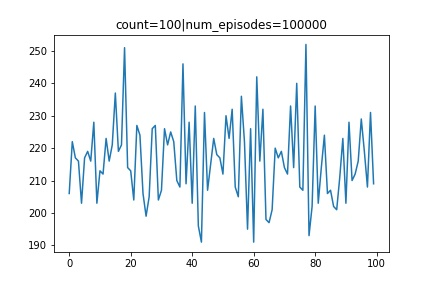
\includegraphics{episodic_reward.jpg}
\end{figure}

\section{\texttt{200Reviews.csv} SVD}

\mybox{In this question, you will employ \textit{Singular Value Decomposition} to obtain word embeddings and compare the generated word embeddings with the word embeddings generated using \texttt{word2vec}. 
The corpus (or dataset) to be considered is "\texttt{200Reviews.csv}". You need to do the following:}

\subsection{Parsing data}
\mybox{Parse the reviews in "\texttt{200Reviews.csv}", i.e., divide reviews into sentences and sentences into words and remove the stop words. You can employ the "\texttt{NLP-pipeline-example.ipynb}" example we talked about in class.}

\textbf{Response:} We import the packages required to process text in our preamble and read the dataframe as shown.

\begin{mdframed}[backgroundcolor=shadecolor]
\begin{minted}[fontsize=\footnotesize,breaklines]{python}
import pandas as pd
import nltk
from nltk.corpus import stopwords
from nltk.stem import WordNetLemmatizer
nltk.download('stopwords')
import re
from textblob import TextBlob
from textblob import Word

df = pd.read_csv(r"200Reviews.csv", encoding = "iso-8859-1")
\end{minted}
\end{mdframed}

Next, we clean the text by replacing obvious mistakes and artifacts using a \texttt{dict}.

\begin{mdframed}[backgroundcolor=shadecolor]
\begin{minted}[fontsize=\footnotesize,breaklines]{python}
replace_dict = {r"`":"",r"â":"a",r'"':"",r"<br />":"",r'\\':""}

for k,v in replace_dict.items():
    df["review"] = df["review"].str.replace(k,v)
for i in range(5):
    df["review"] = df["review"].str.replace(r"  "," ")
\end{minted}
\end{mdframed}

We then tokenize the paragraphs into sentences.

\begin{mdframed}[backgroundcolor=shadecolor]
\begin{minted}[fontsize=\footnotesize,breaklines]{python}
def tokenize_sentences(paragraph):
    return nltk.sent_tokenize(paragraph)

df["review_sentences"] = df["review"].map(tokenize_sentences)
\end{minted}
\end{mdframed}

Defining helper functions that feed into one main function \texttt{process\_text} that corrects spelling, converts text to lower case, removes stopwords, and tokenizes words.

\begin{mdframed}[backgroundcolor=shadecolor]
\begin{minted}[fontsize=\footnotesize,breaklines]{python}
def correct_spelling(word):
    return str(TextBlob(word).correct())

def to_lower(word):
    return word.lower()

def lemmatize(words):
    result = []
    lemmatizer = WordNetLemmatizer()
    for w in words:
        result.append(lemmatizer.lemmatize(w))
    return result

def check_stopword(word):
    stopWords = set(stopwords.words('english'))   
    if word not in stopWords:
        return True
    else:
        return False

def tokenize_word(s):
    wrd_list =  re.split("[^\w]",s)
    tokenized_words = []
    for focus_wrd in wrd_list.copy():
        focus_wrd = focus_wrd.strip()
        if (focus_wrd == ""):
            continue
        if " " in focus_wrd:
            print (focus_wrd)
            tokenized_words.extend(tokenize_word(focus_wrd))
            continue
        tokenized_words.append(focus_wrd)
    return tokenized_words

def process_text(sentences):
    wordlist=[]
    for k in range(len(sentences)):
        words = tokenize_word(sentences[k])    
        words = lemmatize (words) 
        for w in words:            
            w = to_lower(w)            
            if check_stopword(w):
                wordlist.append(w)
    return wordlist

df["review_words"] = df["review_sentences"].map(process_text)
df["new_review"] = df["review_words"].apply(lambda w: " ".join(w))

\end{minted}
\end{mdframed}

The results of the text processing are as follows:

\begin{verbatim}
df['new_review']

0      stuff going moment mj started listening music ...
1      classic war worlds timothy hines entertaining ...
2      film start manager nicholas bell giving welcom...
3      must assumed praised film greatest filmed oper...
4      superbly trashy wondrously unpretentious 80 ex...
                                ...                        
195    collection documentary last 11 minute 9 second...
196    movie ha lot comedy dark gordon liu shine one ...
197    watched kid film year missed come tigers first...
198    probably heard phrase come movie â herbie full...
199    wa thirteen movie came television far superior...
Name: new_review, Length: 200, dtype: object
\end{verbatim}

\subsection{Co-occurence matrix}
\mybox{Create the co-occurrence matrix for all the remaining words (after stop words are eliminated), where the window of co-occurrence is 5 on either side of the word.}

\subsection{Word embeddings}
\mybox{Apply SVD and obtain word embeddings of size 100.  

Then, please generate word embeddings of size 100 using \texttt{Word2Vec.pynb} (from the NLP lecture) on the same "\texttt{200Reviews.csv}" dataset. 
Please show comparison on few examples to understand which method works better. 
Note your observations in your solution.}

\end{document}
